\documentclass[12pt]{article}
\usepackage[top=1in, bottom=1in, left=1in, right=1in]{geometry}

\usepackage{setspace}
\onehalfspacing

\usepackage{amssymb}
%% The amsthm package provides extended theorem environments
\usepackage{amsthm}
\usepackage{epsfig}
\usepackage{times}
\renewcommand{\ttdefault}{cmtt}
\usepackage{amsmath}
\usepackage{graphicx} % for graphics files

% Draw figures yourself
\usepackage{tikz} 

% writing elements
\usepackage{mhchem}

\usepackage{paralist}

% The float package HAS to load before hyperref
\usepackage{float} % for psuedocode formatting
\usepackage{xspace}

% from Denovo Methods Manual
\usepackage{mathrsfs}
\usepackage[mathcal]{euscript}
\usepackage{color}
\usepackage{array}

\usepackage[pdftex]{hyperref}
\usepackage[parfill]{parskip}

% math syntax
\newcommand{\nth}{n\ensuremath{^{\text{th}}} }
\newcommand{\ve}[1]{\ensuremath{\mathbf{#1}}}
\newcommand{\Macro}{\ensuremath{\Sigma}}
\newcommand{\rvec}{\ensuremath{\vec{r}}}
\newcommand{\omvec}{\ensuremath{\hat{\Omega}}}
\newcommand{\vOmega}{\ensuremath{\hat{\Omega}}}
%---------------------------------------------------------------------------
%---------------------------------------------------------------------------
\begin{document}
\begin{center}
{\bf NE 255, Fa16 \\
Simplifying the Transport Equation\\
September 15, 2016}
\end{center}

\setlength{\unitlength}{1in}
\begin{picture}(6,.1) 
\put(0,0) {\line(1,0){6.25}}         
\end{picture}

Recall that last time we created a full version of the transport equation that looked like: 
\begin{align}
&\frac{1}{v}\frac{\partial \psi}{\partial t}(\rvec,E,\omvec,t) + \omvec\cdot  \nabla \psi(\rvec,E,\omvec,t) +
 \Sigma_t(\rvec,E)\psi(\rvec,E,\omvec,t) 
\\& \quad\quad\quad\quad =
\int_0^{\infty}\int_{4\pi}\Sigma_s(\rvec, E'\rightarrow E,\omvec'\rightarrow\omvec)
\psi(\rvec,E',\omvec',t)d\omvec'dE'\nonumber
\\&\quad\quad\quad\quad\quad\quad +\frac{\chi_p(E)}{4\pi}\int_0^{\infty}\int_{4\pi}\nu(E')\Sigma_f(\rvec,E')
\psi(\rvec,E',\omvec',t)d\omvec'dE'\nonumber
\\&\quad\quad\quad\quad\quad\quad\quad\quad+S(\rvec, E, \omvec,t) \nonumber.
\end{align}
What does each term describe?

Today we'll cover some common ways to simplify this equation as well as how to treat scattering.

%----------------------------------------------
\section*{Simplified Forms}
At the end of class we went briefly into simplifications; we're going to spend more time on that in this class. 

\subsection*{Time Independent}
We'll spend most of our time on this version of the equation. We assume that losses and sources are balanced, and thus there is no rate of change with time:
\[\frac{\partial \psi}{\partial t} = 0\]
We can then remove the time dependence from all terms in our equation. As noted, for reactors we often 
\begin{compactitem}
\item solve a steady-state form of the equation,
\item perform depletion calculations that characterize material evolution (using the Batemann equations, which we're skipping for now)
\item solve a new steady-state calculation with updated material specifications.
\end{compactitem}

\subsection*{One Speed}
Assume all particles are at the same speed, $\vec{v} = v_0 \cdot \vOmega$. Thus
\begin{align*}
n(\vec{r}, v, \vOmega, t) &= n(\vec{r}, \vOmega, t) \delta(v - v_0) \\
\Sigma_s(E' \rightarrow E, \vOmega' \rightarrow \vOmega) &= \Sigma_s(E, \vOmega' \rightarrow \vOmega)\delta(E' - E)
\end{align*}
%
Now we can remove E integration and E dependence:
%
\begin{align*}
\frac{1}{v}\frac{\partial \psi(\vec{r}, \vOmega, t)}{\partial t} &+ 
\vOmega \cdot \nabla \psi(\vec{r}, \vOmega, t) +
\Sigma_t \psi(\vec{r}, \vOmega, t) = \nonumber\\
%
& \int_{4\pi} d\vOmega' \Sigma_s(\vOmega' \rightarrow \vOmega) \psi(\vec{r}, \vOmega', t)  
+ \frac{\nu \Sigma_f}{4\pi} \int_{4\pi} d\vOmega' \psi(\vec{r},  \vOmega', t) 
+ S(\vec{r}, \vOmega, t) 
%Q(\vec{r}, \vOmega, t)
\end{align*}
%
%Where:
%\begin{align}
%Q(\vec{r}, \vOmega, t) &= \frac{1}{4\pi} \nu \Sigma_f \int_{4\pi} d\vOmega' \psi(\vec{r},  \vOmega, t) + S(\vec{r}, \vOmega, t) \\
%&= \frac{1}{4\pi} \bigl( \nu \Sigma_f \phi(\vec{r}, t) + s(\vec{r}, t) \bigr)
%\end{align}

\subsection*{Isotropic Source}
It is often the case that an external source is (or we can approximate it as) isotropic:
\[ S(\vec{r}, E, \vOmega, t) = \frac{1}{4 \pi}  S(\vec{r}, E, t) \]


%---------------------------------------------
\subsection*{One Dimensional and Rotational (Azimuthal) Symmetry}
We also often simplify by only worrying about fewer dimensions. Here we'll look at just one: we'll get rid of $x$ and $y$. Let's remind ourselves of how phase-space looks (see \autoref{fig:phase_space}):
\begin{figure}[h!]
    \begin{center}
    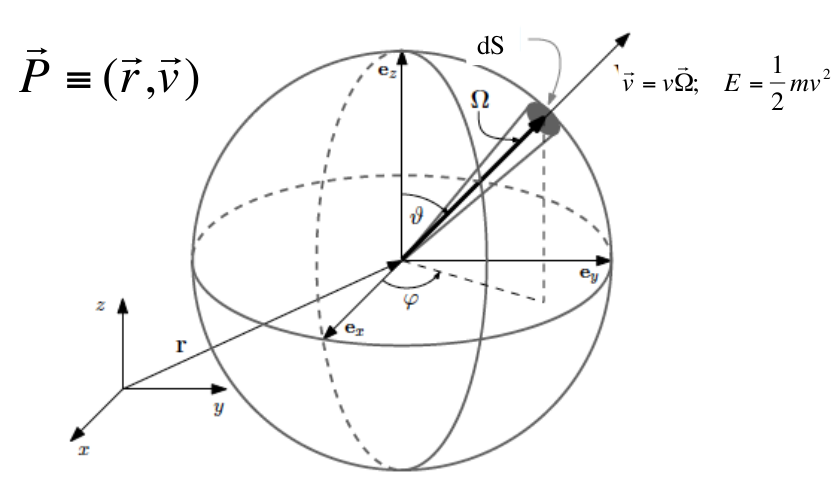
\includegraphics[keepaspectratio, width = 4 in]{phase-space}
    \end{center}
    \caption{Schematic of Phase Space}
    \label{fig:phase_space}
\end{figure}

We first assume that \textbf{things only vary in the $z$ dimension}, so $\vec{r} \rightarrow z$, e.g.\\ $\psi(\vec{r}, E, \vOmega, t) \rightarrow \psi(z, E, \vOmega, t)$

We next assume (which is often true) that our systems is \textbf{azimuthally symmetric}, which means that the scattering is symmetric about the azimuthal direction ($\varphi$). Therefore, scattering only depends on the angle of the scattering cosine, $\mu_0 =\vOmega' \cdot \vOmega$--the angle between where it was heading and where it is heading. We can use this assumption to simplify two things. 

We will use these terms in our simplifications:\\
$d\vOmega = \sin(\theta) d\theta d\varphi = d\mu d\varphi; \quad \mu = \cos(\theta)\,$ so $d\mu = \sin(\theta)d\theta\:; \quad \Omega_z = \cos(\theta) = \mu$ and recall our new definition $\mu_0 = \vOmega' \cdot \vOmega$.
\begin{align*}
\int_{4 \pi} d\vOmega &= \int_0^{2\pi} d\varphi \int_{0}^{\pi} \sin(\theta) d\theta =  \int_0^{2\pi} d\varphi \int_{-1}^1 d\mu = 4\pi \\
\psi(z,\vOmega,E,t) d\vOmega &= \psi(z,\varphi, \mu,E,t) d\varphi  d\mu =  \psi(z, \mu,E,t) d\varphi  d\mu 
\end{align*}
%
With azimuthal symmetry we can rewrite the scattering cross section since it is no longer a function of $\varphi$.
\[\Sigma_s(z, \vOmega' \rightarrow \vOmega) \rightarrow \Sigma_s(z, \vOmega' \cdot \vOmega) = \Sigma_s(z, \mu_0) \:.\]

Further, we can execute the angular integration over $\varphi$ since nothing depends on it anymore. For example:
\[
\int_{4 \pi} d\vOmega\: \psi(z, \vOmega, E, t) =   \int_0^{2\pi} d\varphi \int_{-1}^1 d\mu \:\psi(z, \vOmega, E, t) = 2 \pi \int_{-1}^1 d\mu \:\psi(z, \mu, E, t)\:.\]
%
The next simplification is in the streaming term:
\[\vOmega \cdot \nabla \psi(\vec{r}, \vOmega, E, t) \rightarrow \Omega_z \frac{\partial \psi(z, \mu, E, t)}{\partial z} = \mu \frac{\partial \psi(z, \mu, E, t)}{\partial z} \]
%
We can combine all of this into a 1-D equation, using $\mu_0 = \vOmega' \cdot \vOmega$:
\begin{align*}
\frac{1}{v}\frac{\partial \psi}{\partial t}(z,E,\omvec,t) &+ \Omega_z \frac{\partial \psi(z, \vOmega, E, t)}{\partial z} + \Sigma_t(z)\psi(z, \vOmega, E, t)  \\
&= \frac{\chi(E)}{4 \pi} \int_0^{\infty} dE'\int_{4 \pi} d\vOmega'\:  \nu(E')\Sigma_f(z,E',t)\psi(z, \vOmega', E', t)  \\
&+ \int_0^{\infty} dE' \int_{4 \pi} d\vOmega'\: \Sigma_s(z, \mu_0)\psi(z, \vOmega', E', t) + S(z, E, \vOmega, t)\:,
\end{align*}
%
which we can then integrate over the $\varphi$ component of angle:
\begin{align*}
\frac{1}{v}\frac{\partial \psi}{\partial t}(z,E,\mu,t) &+ \mu \frac{\partial \psi(z, \mu, E, t)}{\partial z} + \Sigma_t(z)\psi(z, \mu, E, t) \\
&= 2\pi\frac{\chi(E)}{4 \pi} \int_0^{\infty} dE' \: \nu(E')\Sigma_f(z,E') \int_{-1}^1 d\mu'\: \psi(z, \mu', E', t) \\
&+ 2\pi\int_0^{\infty} dE' \int_{-1}^1 d\mu'\: \Sigma_s(z, \mu_0)\psi(z, \mu', E', t)  + S(z, E, \mu, t)
\end{align*}
%
Note that the fission terms becomes
\[\frac{\chi(E)}{2} \int_0^{\infty} dE'\:  \nu(E')\Sigma_f(z,E')\underbrace{\phi(z, E', t)}_{\text{scalar flux}}\:. \]

\subsection*{Combination}
If we combine one-speed, time-independent, isotropic source, one-dimensional, and azimuthally-symmetric, we get
\begin{align*}
\mu \frac{\partial \psi(z, \mu)}{\partial z} &+ \Sigma_t(z)\psi(z, \mu) = \\
&\frac{\nu\Sigma_f(z) }{2}\phi(z) + 2\pi\int_{-1}^1 d\mu'\: \Sigma_s(z, \mu_0)\psi(z, \mu')  + \frac{S(z)}{2} \:.
\end{align*}

\subsection*{Scattering}
Our favorite friend, double differential scattering, can be simplified. Let's start by recalling
\[\Sigma_s(\vec{r}, E', \vOmega' \rightarrow E, \vOmega) = \Sigma_s(\vec{r},E') f_s(E', \vOmega' \rightarrow E, \vOmega)\:.\]
We can represent the fractional probability as a product of two independent fractional probabilities (Which is technically an assumption, but is well-supported by reality):
\[f_s(E', \vOmega' \rightarrow E, \vOmega) = f_{sE}(E' \rightarrow E) f_{s\Omega}(\vOmega'  \rightarrow \vOmega)\:.\]
%
In the \textbf{monoenergetic} case, $f_{sE}(E \rightarrow E') = 1$ and with \textbf{isotropic scattering}, $f_{s\Omega}(\vOmega'  \rightarrow \vOmega) = \dfrac{1}{4\pi}$, which would combine to give $\Sigma_s(\vec{r}, E', \vOmega' \rightarrow E, \vOmega) = \dfrac{\Sigma_s(\vec{r})}{4 \pi}$.

If \textbf{scattering is not isotropic}, what do we do? That is,  when we can't simplify so easily, we at least need to represent it in a way we can numerically manage. There are several approaches, but this one makes the most sense to me (different from Duderstadt and Hamilton). 

We expand the scattering cross section in Legendre Polynomials, which are a sequence of orthogonal polynomials:
%
\[P_n(x) = \frac{1}{2^n n!}\frac{d^n}{dx^n} \bigl[\bigl( x^2 -1 \bigr)^n\bigr]\:,\]
as follows
\[\Sigma_s(\vOmega' \cdot \vOmega) = \sum_{l=0}^{\infty} \frac{2l+1}{4\pi} \Sigma_{sl} P_l(\mu_0) = \sum_{l=0}^{\infty} \frac{2l+1}{4\pi} \Sigma_{sl} P_l(\vOmega')P_l(\vOmega) \:. \]
%
(Note that we used the Legendre Addition Thoerem, which uses spherical harmonics. You can learn more here:\\
\hspace*{2em}\href{https://en.wikipedia.org/wiki/Legendre_polynomials}{https://en.wikipedia.org/wiki/Legendre\_polynomials}\\ \hspace*{2em}\href{https://en.wikipedia.org/wiki/Spherical_harmonics}{https://en.wikipedia.org/wiki/Spherical\_harmonics},\\
but for now just note that there are identities and manipulations that allow this to be true). 

Legendre polynomials are solutions to Legendre's differential equations,
\[\frac{d}{dx}\bigl[(1 - x^2) \frac{d}{dx} P_n(x) \bigr] + n(n+1)P_n(x) = 0\:,\]
and are orthogonal on $[-1,1]$:
\begin{gather*}
\int_{-1}^{1}P_n(x)P_m(x)dx = 
\frac{2}{2n+1}\delta_{n,m}= \quad\frac{2}{2n+1}\text{if n = m,} \quad 0\text{ if n $\neq$ m.}\\
\therefore P_0(\mu) = 1 \\
P_1(\mu) = \mu\:.
\end{gather*}
%
We can see the first several polynomials in \autoref{fig:legendre}.
\begin{figure}[h!]
    \begin{center}
    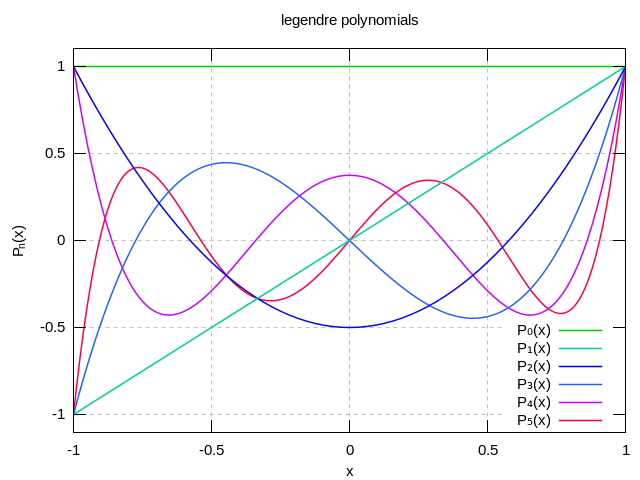
\includegraphics[keepaspectratio, width = 3.5 in]{Legendrepolynomials}
    \end{center}
    \caption{Legendre polynomials}
    \label{fig:legendre}
    %https://en.wikipedia.org/wiki/Legendre_polynomials
\end{figure}

We get the scattering expansion coefficients from the orthogonality of Legendre Polynomials. Any function can be expanded on the interval $-1 \leq x \leq 1$
\[
f(x) = \sum_{l=0}^{\infty} \frac{2n+1}{2} f_n P_n(x)
\]
To find $f_n$, multiply by $P_l$ and integrate over $(-1,1)$:
\begin{align*}
\int_{-1}^1 dx\: f(x) P_l(x) &= \sum_{l=0}^{\infty} \frac{2n+1}{2} f_n\int_{-1}^1 dx\:  P_n(x) P_l(x)\\
\therefore f_l &= \int_{-1}^1 dx\: f(x) P_l(x)\\
\text{and by analogy}\Sigma_{sl} &= 2\pi \int_{-1}^1 d\mu_0 \: P_l(\mu_0)\Sigma_s(\mu_0)\:.
\end{align*}

All of that was to say, we can actually deal with scattering when it's \textit{not} isotropic by expressing the scattering cross section as an expansion in Legendre polynomials. In our simplified transport equation, this looks like:
\begin{align*}
\mu \frac{\partial \psi(z, \mu)}{\partial z} &+ \Sigma_t(z)\psi(z, \mu) = \\
&\frac{\nu\Sigma_f(z) }{2}\phi(z) +  \sum_{l=0}^{\infty} \frac{2l+1}{2} \Sigma_{sl}(z) \int_{-1}^1 d\mu'\: P_l(\mu_0) \psi(z, \mu')  + \frac{S(z)}{2} \:.
\end{align*}
%
In reality, we truncate the expansion at some point. Some common truncations:
\begin{align*}
&l=0 \text{ is isotropic; (note } P_0 (\vOmega) = 1 \text{)}\\
&\qquad \Sigma_s(\vOmega' \cdot \vOmega) \cong \frac{1}{4\pi}\Sigma_{s0} \\
%
&l=1 \text{ is linearly isotropic; (note } P_1 (\vOmega) = \vOmega \text{)}\\
&\qquad \Sigma_s(\vOmega' \cdot \vOmega) \cong \frac{1}{4\pi}\bigl( \Sigma_{s0} + 3\vOmega' \vOmega \Sigma_{s1} \bigr) 
\end{align*}
%
In describing representations of the TE, people commonly describe call out the scattering by saying the $P_n$ expansion of scattering. 



\end{document}
